\section{基于机器视觉的人体运动类型识别}\label{ux57faux4e8eux673aux5668ux89c6ux89c9ux7684ux4ebaux4f53ux8fd0ux52a8ux7c7bux578bux8bc6ux522b}

\subsection{摘要}\label{ux6458ux8981}

本文提出用基于深度学习的机器视觉模型,在只使用由 Kinect
采集回来的人体骨架的运动数据的条件下进行人体运动类型的识别。使用由
Kinect
采集回来骨架模型是因为它具有数据容易获取,数据维度少的特点,可以方便存储、传输。而文章中的这个识别模型在训练时除了
CAD-60
数据集提供的人体骨架数据,没有使用任何的先验知识来进行人体运动类型的识别。这样子可以减少在数据的预处理阶段中人工的干预,只由机器自己来进行特征的提取,这样子可以减少人工提取特征时出现的错误。这也能使最终的模型的泛化性更优秀,鲁棒性更好。从而让模型对人体运动类型有更好的理解与识别。模型上,本文测试了卷积神经网络、自编码器、降噪自编码器、限制玻耳兹曼机以及混合的多种结构,并实验了多种网络训练上的用来加强效果的算法,比如一些正规化的方法和其他新的激活函数,最后选择了卷积神经网络作为自动特征提取的模型,并在其后面配合上多层感知机来进行分类。

关键字:人体运动类型识别,CAD-60
数据集,深度学习,卷积神经网络,自编码器,限制玻耳兹曼机,Kinect

\section{HUMAN ACTION RECOGNITION BASE ON COMPUTER
VISION}\label{human-action-recognition-base-on-computer-vision}

\subsection{Abstract}\label{abstract}

We propose in the paper a computer vision model base on deep learning,
which can recognize the human action only base on the data source in the
skeletons of the human from Kinect. Using the skeletons from Kinect is
because it is easy to get, to store and to transfer, and it has the less
order of the data. This model only use the human skeletons data from the
CAD-60 dataset to recognize the human action without using any prior
knowledge. It can reduce the works from the human on the stage of
preprocessing and hand the feature extraction to the computer, which can
reduce the error from the human-engineer. It can also improve
generalization performance and robustness of the model, And give the a
understanding of the human action. In the paper, we do the experiment on
with convolutional neural networks, autoencoder, denoising autoencoder,
Restricted Boltzmann Machines and the some of their mixture, and it also
do some experiments for the tricks which can improve the nerual network,
such as some regularization methods or other activation functions. In
the end, we choose the convolutional neural networks for the feature
extraction. And use the multilayer perceptron as the follow classifier.

keywords: Human action recognition, CAD-60 dataset, deep models,
convolutional neural networks, autoencoder, Restricted Boltzmann
Machines, Kinect

\subsection{绪论}\label{ux7eeaux8bba}

\subsubsection{引言}\label{ux5f15ux8a00}

计算机自动去理解人类的行为、动作还有跟环境之间的交流互动,在近年来逐渐地成为了一个热门的领域,因为这个技术在很多领域都有可以使用的地方。比如现代社会快速的生活节奏和巨大的工作压力,严重影响着个人的身体健康。科学的运动可以提高身体素质增强运动能力,进而降低患病的风险(尤其是一些慢性疾病),例如糖尿病、血脂异常、高血压等。而进行科学运动的前提是实现人体运动类型的准确识别。
在信息安全领域,通过智能监控的方式利用计算机自动对视频中人体的运动类型进行识别从而为监控或者案件侦破提供依据也具有着重要的意义和广泛的用途。
在人机交互领域可以通过手势、身体姿态等信息对除了辅助交互输入设备以及自然语言分析进行补充,提高计算机和人进行交互的能力,使之更有趣。
在大型的图像数据库或者互联网上的信息中还可以利用人体运动类型的识别,对部分信息进行标注和理解,进而提供搜索和学习的能力。
本课题的任务是通过使用深度学习的相关理论,尝试构造用基于深度学习的机器视觉模型,应用于人体运动类型的识别,从而让模型对人体运动类型有更好的理解与识别。

\subsubsection{人体运动类型识别的相关研究现状}\label{ux4ebaux4f53ux8fd0ux52a8ux7c7bux578bux8bc6ux522bux7684ux76f8ux5173ux7814ux7a76ux73b0ux72b6}

\paragraph{人体运动数据源的获得}\label{ux4ebaux4f53ux8fd0ux52a8ux6570ux636eux6e90ux7684ux83b7ux5f97}

首先,对于人体运动识别的数据的来源存在着几种不同的种类{[}1{]}。例如由
RGB
摄像机、距离传感器或其他遥感的方式。使用深度传感器来进行人体运动识别的发展始于
80
年代初。过去的研究主要集中在学习和认识到从视频序列(可见光相机)所采集的数据中。可见光视频的主要问题是从单目视频传感器捕捉得到的人体运动存在相当大的损失。由于视频天生的对的人体行为识别的限制,尽管已经有了过去几十年的努力,但通过视频来识别人体运动,仍然是非常具有挑战性的。
而得益于近期发布的成本低廉的深度传感器,我们看到了和 3D
数据相关的研究越来越多了。从过去的 20 年里,我们获得 3D
数据的方法,一共分为三类。一种方法是通过使用基于标记的动作捕捉系统,如
MoCap。 第二种方式是通过立体视觉: 从多个角度捕获 2D
图像序列,通过从多个视图来重建三维信息。第三种方式是使用距离传感器(使用类似
TOF
原理的传感器)。深度相机在过去几年里取得迅速的发展。最近出现的深度照相机可以在相对低廉的成本和较小的尺寸里给我们提供较高的帧率和分辨率,这导致出现了许多新的研究中的动作识别都是采用的三维数据。

\paragraph{人体动作识别的主要问题}\label{ux4ebaux4f53ux52a8ux4f5cux8bc6ux522bux7684ux4e3bux8981ux95eeux9898}

基于视觉的人体动作识别里有四个主要的问题。第一个问题的挑战性比较小
{[}2{]} {[}3{]}:闭塞、 杂乱的背景、
阴影和不同光照条件会让运动难以分割或者被错误地识别。这是从 RGB
视频行为识别的一大难点。引入 3D
数据可以在很大程度上通过提供现场的结构信息,从而缓解这个问题。第二个是视角的变换{[}2{]}
{[}4{]} {[}5{]} 和
{[}6{]}。相同的操作可以从不同的角度产生不同的``外观''。传统的 RGB
相机解决这一问题的方法主要是引入多个同步的摄像机,同时获得多个视角的图像,但对于某些应用程序,这不是件容易的事。不过对于三维运动捕捉系统,这不是一个严重的问题。而如果通过深度图像来进行识别的话,这个问题也会有部分被缓解,因为从轻微旋转的视角的外观可以推断深度的信息。这一点并不完全解决问题,因为摄像机始终还只是在对象的一侧上,这个距离图像只提供了部分的信息,还是没有人知道这个对象的另一面是什么样子的。如果可以运用单一深度相机来精确地推断出人的骨架模型,则可以通过骨架模型的信息来构造一种视图不变识别的算法。第三个问题是放缩上的差异,因为人离相机的距离的不同会影响主体的大小从而影响运动的识别。而在
RGB 视频中,这可以通过在多个尺度下的{[}7{]}
特征提取解决了。而在深度视频中,这可以很容易调整,因为真正的主体的 3D
尺寸直接是已知的。第四个问题是同一种类内的变异性和不同种类之间的相似性问题{[}8{]}。人可以通过不同的身体部位在不同的方向上做动作,但不同的方向和两个动作仅只有只由非常细微的细节来区分。而这个不管对于使用哪种数据的来源的算法来说都仍然是一个非常困难的问题。\\前三个问题基本上都可以通过使用三维空间上的图像或者类似骨架之类的模型来解决,所以本文使用的数据来源是由传感器采集计算直接得到的骨架数据。

\paragraph{人体动作识别的相关研究成果}\label{ux4ebaux4f53ux52a8ux4f5cux8bc6ux522bux7684ux76f8ux5173ux7814ux7a76ux6210ux679c}

从各种论文来看,相关研究的重点都是集中在寻找合适的特征,如时空趣点特征STIP{[}9{]}、骨架模型{[}9{]}{[}10{]}{[}11{]}、方向梯度直方图(HOG:Histogram
of oriented gradients){[}12{]}{[}13{]} 、
光流场方向直方图(HOF:Histograms of Optical
Flow){[}12{]}{[}14{]}{[}15{]}、EigenJoints{[}16{]}等特征或者是它们的一些拓展和变形,如方向HOF{[}17{]},以及根据这些特征进行进一步的组合来产生更高级的特征。\\然后把这些特征通过分类器如贝叶斯模型{[}16{]}{[}18{]}、k近邻kNN{[}19{]}、支持向量机
SVM{[}12{]}{[}19{]}{[}20{]}{[}14{]}{[}21{]}{[}22{]}、隐马尔可夫模型
HMM{[}19{]}{[}11{]}来进行有监督的学习得到分类。分类器之间也可以通过串联{[}16{]}或者并联(票决、加权)来加强分类的效果。

\paragraph{使用深度学习进行有效的特征提取}\label{ux4f7fux7528ux6df1ux5ea6ux5b66ux4e60ux8fdbux884cux6709ux6548ux7684ux7279ux5f81ux63d0ux53d6}

上一节所说到的特征的选取或者是计算一般是通过人工方式得到的。而这种人工方式得到的特征对应用的领域有较强的依赖性,也就是说,换一个研究的问题之后可能同样的特征就不能再适用了。\\而深度学习{[}23{]}的提出,某种程度上解决了这些关于特征提取的这些问题。
模仿出人脑表征信息的高效和鲁棒性一直是近几十年来人工智能研究中的一个核心。而人类不仅每时每刻都暴露在由感官接收的无数的数据中,而且还能够通过某些方法捕捉到这些数据关键的部分来让自己能够以简单的方式在未来使用。早在五十年前,提出了动态规划理论以及开创了最优化控制领域的
Richard Bellman
就曾断言,数据的高维度是在人工智能科学和工程应用中的根本障碍。其中主要的困难,尤其是在模式分类的应用中,就是数据学习的难度会随着数据维度的线性增长,发生指数级的增长{[}24{]}。而克服这个问题的主流方法就是以一定的方式(比如分类器、SIFT
算法)对数据进行预处理来减少数据的维度,这样数据就可以被有效地处理。这种减少维度的做法一般被称为特征提取。因此,可以认为,在很多模式识别系统的背后的智能其实被转移到了人工的特征提取处理上去了,而这种人工的做法有时会很困难而且会高度依赖于具体的应用场景{[}25{]}。此外,如果不完整或者错误的特征被提取出来了,那么分类处理的性能就会从根本上受到限制。
最近,神经科学在哺乳类动物大脑上的新发现告诉我们,我们可以通过一个复杂的深层网络结构来对数据自动地进行预处理。这就是深度学习的基本来源。

\subsection{特征提取}\label{ux7279ux5f81ux63d0ux53d6}

得益于 Microsoft Kinect 的发布,通过它采集、处理 RGB-D
图像并提取出人体骨架模型的做法已经非常的流行,而且它也能有效地对原数据进行了第一步的特征提取,所以本文的算法是基于由
Kinect
采集出来的人体骨架数据来进行研究的。\\在这一章里,我们先是总结了几种特征提取的模式,然后主要阐述了一些用来对原数据进行非人工的特征提取的方法,并对各种方式进行了实验,列出了对比的数据,最终选择了卷积神经网络来进行特征的自动提取。

\subsubsection{特征提取模式}\label{ux7279ux5f81ux63d0ux53d6ux6a21ux5f0f}

\paragraph{人工特征提取}\label{ux4ebaux5de5ux7279ux5f81ux63d0ux53d6}

这种模式是指是使用一些人工设计的,由人对源数据的理解所构造的算法来进行特征提取如之前说过的骨架模型、时空特征点之类的方法。也就是在识别的模型里加入一些人对数据的理解的先验的知识来加强模型的效果。这种方式会随着不同的数据或者不同的应用领域而改变,每换一个领域可能都需要使用人的知识和能力来进行学习、归纳和总结,然后选择一个特征提取的方式,如下图所示\\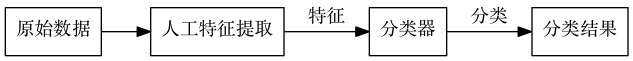
\includegraphics{picture/learning-framework1.png}\\图1.人工特征提取

\paragraph{无监督学习特征提取}\label{ux65e0ux76d1ux7763ux5b66ux4e60ux7279ux5f81ux63d0ux53d6}

这个类型主要是使用无监督学习的方法如限制玻耳兹曼机
RBM,自编码器,或者一些类似主要成分分析 PCA
的算法,在不需要数据集带有标签的前提下能够对数据的特征进行提取,发现特征内在的信息,从而减少数据的冗余,减少数据的维度。而这类型的模式如下图所示\\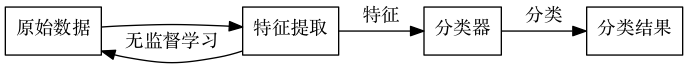
\includegraphics{picture/learning-framework2.png}\\图2.无监督特征提取

\paragraph{有监督特征提取}\label{ux6709ux76d1ux7763ux7279ux5f81ux63d0ux53d6}

这个类型是使用有监督学习的方法,在特征提取里面把标签的信息也考虑进去,从而使特征提取的结果更有针对性,对后面的分类更有利,这类型里的算法有
CNN
卷积神经网络,过程则如下图所示\\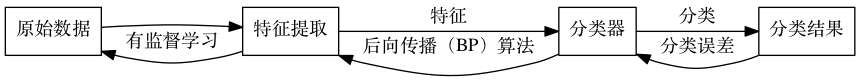
\includegraphics{picture/learning-framework3.png}\\图3.有监督特征提取

\subsubsection{特征提取模型}\label{ux7279ux5f81ux63d0ux53d6ux6a21ux578b}

\paragraph{主要成分分析
PCA}\label{ux4e3bux8981ux6210ux5206ux5206ux6790-pca}

主要成分分析{[}26{]}{[}27{]}
里的假设是,在数据里变化最大的那些因素就是最有价值的因素,因此,只要把输入的数据的空间找到一个变换,这个变换可以把数据里变化最大的因素提取出来,其他变化不那么大(利用价值比较小)的舍弃不看,就可以降低数据的维度,从而减少后面的计算的难度了。\\首先要做的是数据的预处理,也就是数据的均值中心化和方差归一化:\\1.数据的均值中心化,也就是把数值变化范围的中心移至
0
处:\\\[ x^{(i)} = x^{(i)} - \mu = x^{(i)} - \frac{1}{m} \sum_{i=1}^m {x^{(i)}}\]
2.数据的方差归一化:\\\[ x_j^{(i)} = x_j^{(i)} / \sigma_j = x_j^{(i)} / \sqrt{\frac{1}{m} \sum_{i=1}^m {(x_{j}^{(i)})^2}} \]

然后进行 PCA 核心环节:\\1.首先求协方差矩阵:
\[\sum = \frac{1}{m} \sum_{i=1}^{m}(x^{(i)})(x^{(i)})^T\]
2.求得协方差矩阵的特征向量\(U\)并按特征值\(\lambda_n\)从大到小依次排列得到:\\\[U=[u_1 u_2 .... u_n]\]
3.按照一定的方法取 \(k\) ,比如一个常见的经验法则是选择 \(k\)
以保留99\%的方差:
\[\frac{\sum^{k}_{j=1}\lambda_j}{\sum^{n}_{j=1}\lambda_j} >= 0.99\]\\4.取前
\(k\) 个特征值对应的特征向量,组成新的特征向量矩阵\(U'\)。并与 \(x\)
相乘,得到新的降维后的数据 \(x'\):\\\[U' = [u_1 u_2 .... u_k]\]
\[x' = U'^T * x\]

\paragraph{自编码器
Autoencoders}\label{ux81eaux7f16ux7801ux5668-autoencoders}

一个自编码器{[}28{]}{[}29{]}会对一个输入 \(x∈[0, 1]^{d}\)
经过一次线性变换之后得到一个确定的表达 \(y∈[0,1]^{d′}\)
:\\\[y = s(Wx + b)\]\\这其中的 \(s\) 是非线性环节,比如 sigmoid
函数。然后,这个潜在的对输入的表达 \(y\)
(或者说编码),会被再一次地重新映射(或者说解码)到一个和 \(x\)
一样结构大小的重建出来的
\(z\)。(上述的式子没有使用矩阵变换的形式)。这里的 \(z\) 应该视为在
\(y\) 的表达下的 \(x\) 的一种预测。而重建的里面的 \(W'\)
可以限制为正向映射的 \(W\) 的倒置:\(W'=W^T\)。而这个模型的参数(比如
\(W',b,b'\))可以通过使平均重建误差最小化来进行优化。\\重建误差可以通过很多方法进行测量,这个依赖于编码的输入的分布。传统的\\\[L(xz) = ||x-z||^2\]\\也是可以使用的。\\这里面的
\(y\)
是输入的数据的空间中的主要因子的一个表达。这个跟主要成分分析中的捕捉输入数据空间的主要因子非常类似。而事实上,如果中间的隐含层(编码)是一个线性变换而且是使用均方误差来训练网络的话,有
\(k\) 个隐含单元就意味着其实是在找出原数据的前 \(k\)
主要成分。但是如果隐含层是非线性的话,自编码器就跟 PCA
很不一样了,因为它还具备了捕捉输入数据里多模态的部分。

\paragraph{卷积神经网络}\label{ux5377ux79efux795eux7ecfux7f51ux7edc}

卷积神经网络 CNNs
{[}30{]}{[}31{]}是一个专门为二维数据(例如图片和视频)设计的多层神经网络的系列。
CNNs
是第一种真正意义上成功的深度学习方法,它能够成功地用一种鲁棒的方式训练出多层的神经网络。相比起普通的多层神经网络,卷积神经网络有很多独有的特点。

\subparagraph{稀疏连接}\label{ux7a00ux758fux8fdeux63a5}

卷积神经网络利用了空间的局部相关性,相邻两层之间只进行了局部的连接,而不是像多层感知机
MLP 一样使用全连接的方式。换句话说,隐层 m 的单元的输入来自于层 m-1
在空间上连续的感受野的单位的一个子集。具体的如下图所示:\\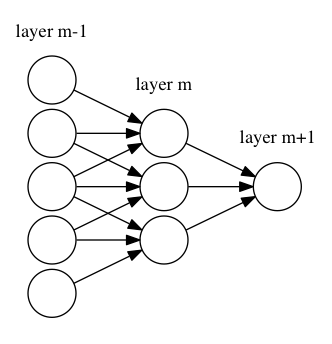
\includegraphics{picture/sparse-connectivity.png}\\图4.稀疏连接

想象一下,层 m-1 是输入,而在上面的图中,层 m 的单位感受野宽度为 3
,因此层 m 的每个神经元只连接到输入层的 3 个相邻的神经元。在层 m+1
中也有与下方图层类似的连接性。我们说他们的感受野宽度也是
3,但实际上他们相对于输入的层 m-1 的感受野的是 5。就是说每个 层m
里的单元都会响应在其关于视网膜的感受野的变化。这个层级结构确保了学习出来的
filter
可以对来自于局部空间的输入产生最强烈的反应。因此,也正如上面所说的,叠加这种层级的结构会导致(非线性)的
filter,可以使它越到后面的层,响应对应的输入感受野更大。例如,在隐藏图层
m + 1 单元可以编码 5 宽度 (以像素的空间)
的非线性特征。\\这种连接的编码方式,比起普通的全连接的神经网络显然可以有效地减少连接的数量,从而能容纳更多的层数,对输入的数据进行更复杂的描述,加强了模型的表达能力。而且,只与上一层的相邻的局部的几个神经元连接的方式,可以使模型具备一定程度的某维度维度上的不变性。

\subparagraph{共享权值}\label{ux5171ux4eabux6743ux503c}

除了稀疏连接之外,每一个 filter
都是一套参数应用在整个输入空间上的。具体如图所示,\\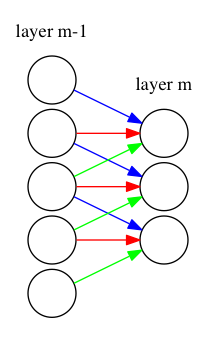
\includegraphics{picture/shared-weights.png}\\图5.权值共享\\红色、蓝色、绿色三种线代表三个权值(W、b,即权值和偏置),层
m
中每个单元都是由相同的这个三个权值和他们对应的感受野里的输入神经元计算出来的。假如没有权值共享,则需要的权值就有
\(3 * 3 = 9\)
个,由此可见,权值共享使得需要进行优化的参数大大地减少了,使得我们能够更有效地进行特征提取。通过控制模型的规模,卷积网络对视觉问题的泛化能力非常好。

\subparagraph{池化(pooling)}\label{ux6c60ux5316pooling}

以上两个特点都是由通过使用卷积核卷积计算生成多个特征图的方式实现的。而完整的卷积神经网络的结构里,还有池化的层用来进行二次的采样,比如使用一个
\(N*N\)
的求最大值窗口或者平均值窗口进行降采样。这种操作被称为池化,池化的操作的作用是可以提供一定的空间位移的不变性以及进一步减少数据的维度,一般池化之后会通过一个激活函数得到一个新的网络的层。

\subparagraph{完整模型}\label{ux5b8cux6574ux6a21ux578b}

以上两个特点都是由通过使用卷积核卷积计算生成多个特征图的方式实现的。而完整的卷积神经网络的结构里,还有其他的东西,以
LeNet为例,展示一下完整的卷积神经网络的结构。\\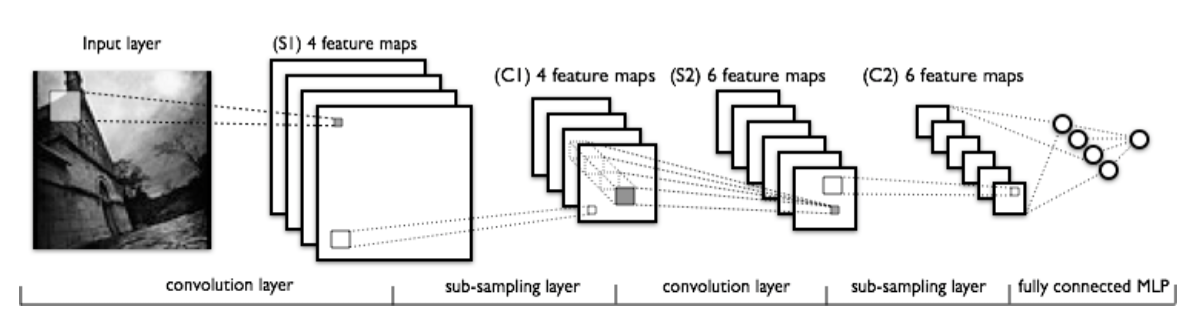
\includegraphics{picture/lenet.png}\\图6.LeNet-网路\\上图中的网络输入图像通过
4 个可训练的滤波器和偏置在 S1 的位置产生了 4
个特征图。特征图中的每个图通过池化并通过一个激活函数之后得到一个 C1
位置上的 4 个新的特征图。然后会通过一个新的卷积层然后得到新的 6 个特征图
S2。这些将再一次池化得到
C2。最终这些像素的值进行光栅化、摊平成一个向量,这个向量就是这个网络里提取得到的特征。这些特征之后就可以输入到一个常规的分类器里,比如神经网络(多层感知机
MLP)里,最终由这个分类器进行分类结果的计算和输出。\\而这些卷积核的权值和偏置,还有其他用到的权值则使用后向传播算法来进行计算出梯度,然后通过梯度下降法之类的算法进行优化,从而训练出来一个有效的特征提取的卷积神经网络。

\subsection{多层感知机(MLP)}\label{ux591aux5c42ux611fux77e5ux673amlp}

特征提取完了之后,需要把特征交到后面的分类器进行分类,而由于有监督的特征提取网络需要得到分类错误后的传递过来的误差,所以需要需要使用可以进行后向传播的分类器,这里面比较经典的分类器就是多层感知机(MLP)也就是普通的神经网络{[}32{]}。

神经网路由神经元组成:\\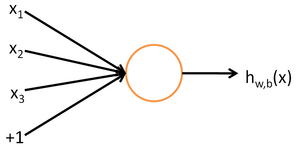
\includegraphics{picture/single-neuron.png}\\图7.典型神经网络中的神经元\\上图中的神经元实际上是一个以
\(x_1, x_2, x_3\) 及截距 \(+1\) 为输入值的运算单元,其输出为
\(h_{W,b}(x) = f(W^Tx) = f(\sum_{i=1}^3 W_{i}x_i +b)\) ,其中函数 \(f\)
被称为``激活函数''。激活函数的作用主要是为神经网络引入非线性环节,使其对非线性的函数具有更好的拟合能力。一般我们会选用
sigmoid 函数作为激活函数:\\\[f(z) = \frac{1}{1+\exp(-z)}\]

典型的神经网络如图所示:\\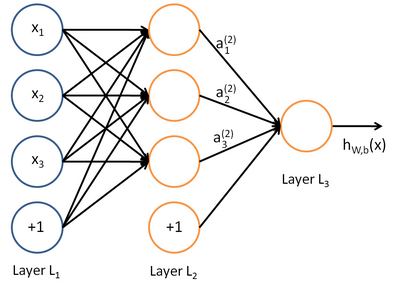
\includegraphics{picture/MLP.png}\\图8.典型多层神经网网络\\如上图所示,把多个神经元按上图的形式以多层的形式串联起来,就可以得到可以一个神经网络用来对数据进行学习、拟合或者分类。

\subsubsection{前向传播}\label{ux524dux5411ux4f20ux64ad}

输入的值经过一层一层的神经元的计算、激活,一直到达最后一层,并得到值称之为前向传播,对于图
8
中的模型,前向传播的计算步骤如下所示:\\\[ a_1^{(2)} = f(W_{11}^{(1)}x_1 + W_{12}^{(1)} x_2 + W_{13}^{(1)} x_3 + b_1^{(1)})\]
\[ a_2^{(2)} = f(W_{21}^{(1)}x_1 + W_{22}^{(1)} x_2 + W_{23}^{(1)} x_3 + b_2^{(1)})\]
\[ a_3^{(2)} = f(W_{31}^{(1)}x_1 + W_{32}^{(1)} x_2 + W_{33}^{(1)} x_3 + b_3^{(1)})\]
\[ h_{W,b}(x) = a_1^{(3)} =  f(W_{11}^{(2)}a_1^{(2)} + W_{12}^{(2)} a_2^{(2)} + W_{13}^{(2)} a_3^{(2)} + b_1^{(2)}\]\\如果把权值
W 表示为矩阵,且将激活函数 \(f()\)
扩展为使用向量则上列等式可以更加简洁地表示为:\\\[z^{(2)} = W^{(1)}x + b^{(1)}\]
\[a^{(2)} = f(z^{(2)})\] \[z^{(3)} = W^{(2)} a^{(2)} + b^{(2)}\]
\[h_{W,b}(x) = a^{(3)} = f(z^{(3)})\]

\subsubsection{后向传播}\label{ux540eux5411ux4f20ux64ad}

上述的前向传递是根据输入,通过网络逐层计算出来合适的结果,但是网络的里的权值、偏置需要确定,所以可以通过梯度下降法来进行对这些参数,也就是对神经网络进行求解。而对于单个输入的测试样例
\((x,y)\),其代价函数为:
\[J(W,b; x,y) = \frac{1}{2} || h_{W,b}(x) - y ||^2\]\\只要得到每一个参数的关于代价函数的偏导数,我们就可以使用梯度下降法来进行优化。\\而求解每一个参数的偏导数就需要使用反向传播算法了。\\反向传播算法的思路如下:给定一个样例
\((x,y)\),我们首先进行``前向传播''运算,计算出网络中所有的激活值,包括
\(h_{W,b}(x)\) 的输出值。之后,针对第 \(l\) 层的每一个节点
\(i\),我们计算出其``残差'' \(\delta^{(l)}_i\)
,该残差表明了该节点对最终输出值的残差产生了多少影响。对于最终的输出节点,我们可以直接算出网络产生的激活值与实际值之间的差距,我们将这个差距定义为
\(\delta^{(n_l)}_i\) (第 \(n_l\)
层表示输出层)。对于隐藏单元我们将基于节点(第 \(l+1\)
层节点)残差的加权平均值计算 \(\delta^{(l)}_i\) ,这些节点以
\(a^{(l)}_i\)
作为输入。\\后向传播算法可以具体表示为以下步骤:\\1.进行前馈传导计算,利用前向传导公式,得到
\(L_2, L_3, \ldots\) 直到输出层 \(L_{n_l}\) 的激活值。\\2.对输出层(第
\(n_l\) 层),计算:
\[\delta^{(n_l)} = - (y - a^{(n_l)}) \bullet f'(z^{(n_l)})\] 3.对于
\(l=n_l-1, n_l-2, n_l-3, \ldots, 2\) 的各层,计算:
\[\delta^{(l)} = \left((W^{(l)})^T \delta^{(l+1)}\right) \bullet f'(z^{(l)})\]
4.计算最终需要的偏导数值:
\[\nabla_{W^{(l)}} J(W,b;x,y) = \delta^{(l+1)}(a^{(l)})^T,\]
\[\nabla_{b^{(l)}} J(W,b;x,y) = \delta^{(l+1)}.\]

\subsection{实验}\label{ux5b9eux9a8c}

本章中,首先会介绍一些我们在实验过程中使用的一些能够增强模型效果、速度、泛化能力的技巧,然后会结合编程实践给出一些编程框架的对比,以及不同算法下的准确率的比较。

\subsubsection{神经网络使用技巧}\label{ux795eux7ecfux7f51ux7edcux4f7fux7528ux6280ux5de7}

\paragraph{数据、网络预处理{[}33{]}}\label{ux6570ux636eux7f51ux7edcux9884ux5904ux7406lecun2012}

\subparagraph{对输入数据进行标准化}\label{ux5bf9ux8f93ux5165ux6570ux636eux8fdbux884cux6807ux51c6ux5316}

由于学习率对于每一个参数都是一样的,所以为了加快收敛,可以让所有参数都以相同的标准进行线性变换,映射到一个一致的范围里对输入的。具体的变换要求如下:\\A、训练集的每个输入变量的均值要接近于0;\\B、对输入变量进行缩放,使他们的方差具有相同的值;\\C、输入变量最好是不相关的。\\如图所示:\\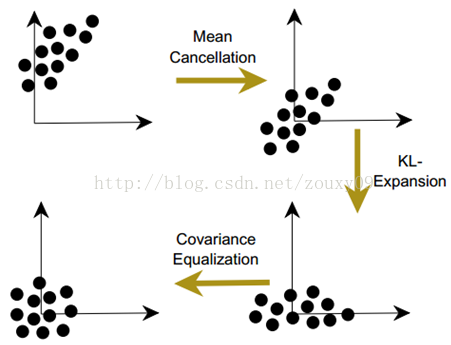
\includegraphics{picture/normalizing-the-inputs.png}\\图9.输入标准化

\subparagraph{参数的初始化}\label{ux53c2ux6570ux7684ux521dux59cbux5316}

参数的初始值对训练过程有着重大的影响。我们对参数初始化的原则是:参数应该随机初始化在能让
sigmoid
函数在线性区域激活的值。如果参数全部都很大,那sigmoid一开始就饱和了,这样就会得到一个非常小的梯度值,那参数更新就会很慢,训练也会很慢。使
sigmoid 函数工作在线性区域激活除了需要输入数据标准化到其标准差为
1,还需要参数初始值,也就是连接神经元的权值的初始值的标准差也能为
1。最简单的做法就是,给参数初始化的时候使用正态分布采样得到,那么参数就会均值为零,且方差近似1。

\subparagraph{打乱样本的学习顺序}\label{ux6253ux4e71ux6837ux672cux7684ux5b66ux4e60ux987aux5e8f}

在使用后向传播算法进行学习的时候,有一个原则是使用意料之外的样本来学习,收敛得会更快。一般来说,训练用的数据都会是规整的,按顺序排列的,比如我们使用的数据集里,人体的运动都是按照时间顺序在一个大的视频里分别进行切片的,所以相邻的训练数据有很大可能是来自于同一个类型甚至是同一个视频的。而这一节的这个技巧就是在粗糙地选择来自不同类的样本,也就是说,尽量让每一次的训练采用的样本都来自不一样的类型,最简单的做法就是把样本的顺序打乱。因为同一个类的训练样本很大可能携带的是相似的信息,而相似的信息很有可能让网络落入一个局部的最优解处。所以为了提高模型的泛化性能,每次使用来进行训练的样本最好是随机地而不是按照顺序地进行选择。

\subsubsection{网络设计技巧}\label{ux7f51ux7edcux8bbeux8ba1ux6280ux5de7}

\paragraph{加入正规化环节防止过拟合}\label{ux52a0ux5165ux6b63ux89c4ux5316ux73afux8282ux9632ux6b62ux8fc7ux62dfux5408}

在模型中加入正规化(Regularization)环节可以避免模型拟合出来的分类面高度非线性,从而避免过拟合现象。过拟合(Overfitting)是指模型对训练数据集中的样本拟合的非常好,但是面对训练集中没有的数据样本的分辨效果很差。正规化的主要实现方式是用某些方法尽量地使参与优化的参数尽可能的小。之所以要让参数尽可能的小,是因为正如下图所示,模型越复杂,就会像右边的图上所示,能拟合任何函数,但是显然已经过拟合了,有可能对新的数据产生分类错误。因此只要参数变小,就可以抑制模型的复杂程度,从而使得模型的泛化能力更强。\\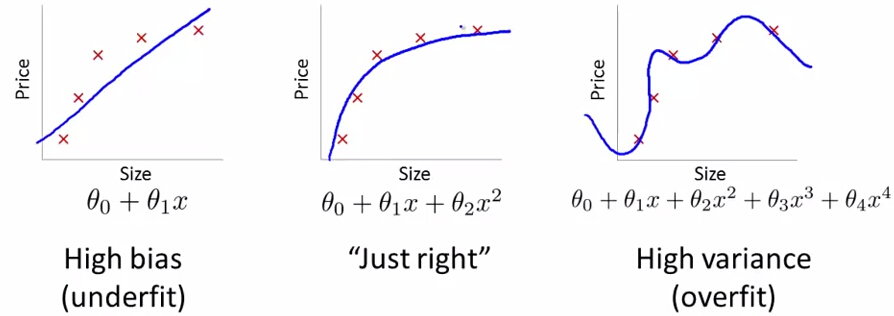
\includegraphics{picture/overfit.jpg}\\图10.过拟合

\subparagraph{加入范数惩罚}\label{ux52a0ux5165ux8303ux6570ux60e9ux7f5a}

而常用的正规化的方法是直接将所有参数 \(θ\)
按某种形式加到最小化目标函数中加以惩罚,以免参数过大导致过拟合现象的产生,比如计算出来参数的
L1、L2范数然后直接把这一项加入到需要被优化的目标函数里去:
\[w = arg min_m\sum L(y_i,f(x_i;w))+\lambda \Omega(w)\]\\一般来说,监督学习可以看作是最小化上面的目标函数,而里面的
\(L(y_i,f(x_i;w))\) 是样本的预测的误差,后面的 \(\Omega(w)\)
就是我们加入的可以用来使模型更简单的正规化函数,比如L1范数正规化的话,有:
\[\Omega(w) = ||w||_1 = \sum|w_i|\]\\使用 L1
范数的正规化的话,还可以实现特征的稀疏表达。\\这个方法里的 \(\lambda\)
需要通过人工设定,可以通过实验来进行选择。

\subparagraph{Max-norm}\label{max-norm}

除了上述的,通过在优化的目标函数里加入权值的范数来进行整个权值空间的惩罚以外,一种有效的正规化方法是
Max-norm。这种算法是在每个单个的隐藏单元里设置这个单元的传入的权值的 L2
范数的上限,如果权值的更新违反了这个约束,我们就可以通过让这些权值除以这个范数来达到让这个权值重新正规化的目的。使用这个约束而不是使用惩罚的方法可以在无论每次权值更新得有多大的情况下防止权值变得非常大。而且,比起惩罚方法,使用约束的时候也可以使一开始的学习率可以取得很大,使得对权值空间的搜索可以更快,更彻底。当然,在这个算法里也有需要人工设置的参数,就是所使用的
L2 范数的上限。

\subparagraph{Dropout}\label{dropout}

正规化的方法中,也有上述方法的变形。比如在网络的训练过程中使用的
Dropout{[}34{]}{[}35{]}算法。可以有效地加强模型的泛化能力,抑制神经网络出现过拟合的现象。\\Dropout
是指在模型训练时随机让网络某些隐含层节点的权值不工作,不工作的那些节点可以暂时认为不是网络结构的一部分,但是它的权值得保留下来(只是暂时这一轮里面它的值不更新而已),下次样本输入时它可能又会恢复工作了。但是这种方法是只适合于训练样本较少的条件下的用来增强模型的泛化能力的。\\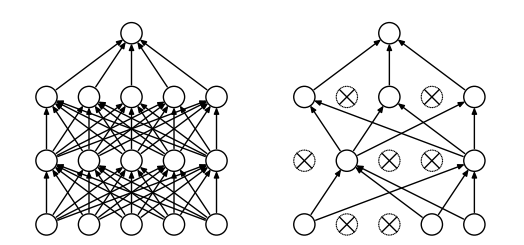
\includegraphics{picture/dropout.png}\\图11.左:标准神经网络;右:使用了
Dropout
算法之后\\而这个算法里需要人工调整的是让某些节点权值不工作的概率,一般会直接选择
50\%。

\paragraph{Maxout}\label{maxout}

Maxout
模型是类似多层感知机、卷积神经网络这种简单的前馈的架构使用的新型的激活函数。对于给定的输入
\(x ∈ \Re\)(x 可能是 \(v\)
或者是某一个隐含层的状态)。\\\[h_i = {max}\limits_{j∈[1,k]}z_{ij}\]
使用 Maxout {[}36{]}
函数来作为激活函数可以加强模型对非线性函数的拟合能力。\\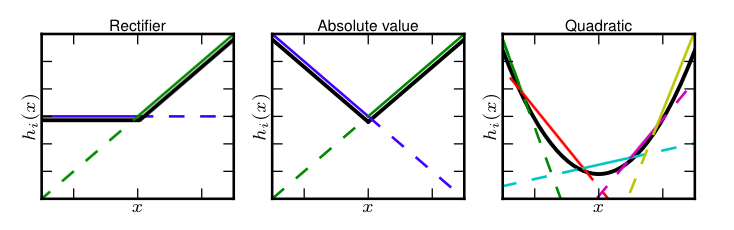
\includegraphics{picture/maxout.png}\\图12.Maxout可以拟合任意凸函数

\paragraph*{引用文献}\label{ux5f15ux7528ux6587ux732e}
\addcontentsline{toc}{paragraph}{引用文献}

{[}1{]}L. Chen, H. Wei, and J. Ferryman, ``A survey of human motion
analysis using depth imagery,'' \emph{Pattern Recognition Letters}, vol.
34, no. 15, pp. 1995--2006, 2013.

{[}2{]}D. Weinland, M. Özuysal, and P. Fua, ``Making action recognition
robust to occlusions and viewpoint changes,'' in \emph{Lecture notes in
computer science (including subseries lecture notes in artificial
intelligence and lecture notes in bioinformatics)}, 2010, vol. 6313
LNCS, pp. 635--648.

{[}3{]}L.-c. Chen, J.-w. Hsieh, C.-h. Chuang, C.-y. Huang, and D. Y.
Chen, ``Occluded Human Action Analysis Using Dynamic Manifold Model,''
in \emph{International conference on pattern recognition}, 2012, pp.
1245--1248.

{[}4{]}M. B. Holte, T. B. Moeslund, N. Nikolaidis, and I. Pitas, ``3D
Human Action Recognition for Multi-view Camera Systems,'' in \emph{2011
international conference on 3D imaging, modeling, processing,
visualization and transmission}, 2011, pp. 342--349.

{[}5{]}D. Weinland, E. Boyer, and R. Ronfard, ``Action recognition from
arbitrary views using 3D exemplars,'' in \emph{Proceedings of the iEEE
international conference on computer vision}, 2007, pp. 1--7.

{[}6{]}M. C. Roh, H. K. Shin, and S. W. Lee, ``View-independent human
action recognition with Volume Motion Template on single stereo
camera,'' \emph{Pattern Recognition Letters}, vol. 31, no. 7, pp.
639--647, 2010.

{[}7{]}M.-y. Chen, ``MoSIFT : Recognizing Human Actions in Surveillance
Videos MoSIFT : Recognizing Human Actions in Surveillance Videos.''
2009.

{[}8{]}R. Poppe, ``A survey on vision-based human action recognition,''
\emph{Image and Vision Computing}, vol. 28, no. 6, pp. 976--990, 2010.

{[}9{]}Y. Zhu, W. Chen, and G. Guo, ``Evaluating spatiotemporal interest
point features for depth-based action recognition,'' \emph{Image and
Vision Computing}, vol. 32, no. 8, pp. 453--464, 2014.

{[}10{]}L. Piyathilaka and S. Kodagoda, ``Gaussian mixture based HMM for
human daily activity recognition using 3D skeleton features,''
\emph{Proceedings of the 2013 IEEE 8th Conference on Industrial
Electronics and Applications, ICIEA 2013}, pp. 567--572, 2013.

{[}11{]}S. Gaglio, G. L. Re, S. Member, and M. Morana, ``Human Activity
Recognition Process Using 3-D Posture Data,'' pp. 1--12, 2014.

{[}12{]}L. Rybok, B. Schauerte, Z. Al-Halah, and R. Stiefelhagen,
```Important stuff, everywhere!' Activity recognition with salient
proto-objects as context,'' \emph{2014 IEEE Winter Conference on
Applications of Computer Vision, WACV 2014}, pp. 646--651, 2014.

{[}13{]}N. Dalal and B. Triggs, ``Histograms of oriented gradients for
human detection,'' in \emph{Proceedings - 2005 iEEE computer society
conference on computer vision and pattern recognition, cVPR 2005}, 2005,
vol. I, pp. 886--893.

{[}14{]}B. Ni, Y. Pei, P. Moulin, and S. Yan, ``Multilevel depth and
image fusion for human activity detection,'' \emph{IEEE Transactions on
Cybernetics}, vol. 43, no. 5, pp. 1382--1394, 2013.

{[}15{]}R. Chaudhry, a. Ravichandran, G. Hager, and R. Vidal,
``Histograms of oriented optical flow and Binet-Cauchy kernels on
nonlinear dynamical systems for the recognition of human actions,''
\emph{2009 IEEE Conference on Computer Vision and Pattern Recognition},
pp. 1932--1939, 2009.

{[}16{]}X. Yang and Y. Tian, ``Effective 3D action recognition using
EigenJoints,'' \emph{Journal of Visual Communication and Image
Representation}, vol. 25, no. 1, pp. 2--11, 2014.

{[}17{]}K. Lertniphonphan, S. Aramvith, and T. H. Chalidabhongse,
``Human action recognition using direction histograms of optical flow,''
\emph{2011 11th International Symposium on Communications \& Information
Technologies (ISCIT)}, vol. c, no. Iscit, pp. 574--579, 2011.

{[}18{]}D. R. Faria, C. Premebida, and U. Nunes, ``A Probabilistic
Approach for Human Everyday Activities Recognition using Body Motion
from RGB-D Images,'' \emph{IEEE International Symposium on Robot and
Human Interactive Communication (Ro-Man)}, 2014.

{[}19{]}J. Shan and S. Akella, ``3D Human Action Segmentation and
Recognition using Pose Kinetic Energy,'' 2014.

{[}20{]}N. Hu, G. Englebienne, Z. Lou, and B. Kr, ``Learning Latent
Structure for Activity Recognition *,'' pp. 1048--1053, 2014.

{[}21{]}C. Zhang and Y. Tian, ``RGB-D camera-based activity analysis,''
\emph{\ldots{}and Conference (APSIPA ASC), 2012 Asia- \ldots{}}, 2012.

{[}22{]}J. Sung, C. Ponce, B. Selman, and A. Saxena, ``Human Activity
Detection from RGBD Images,'' 2011.

{[}23{]}I. Arel, D. C. Rose, and T. P. Karnowski, ``Deep Machine
Learning --- A New Frontier in Artificial Intelligence Research,''
\emph{IEEE Computational Inteligence Magazine}, vol. 5, no. 4, pp.
13--18, 2010.

{[}24{]}R. E. Bellman, \emph{Chapter 6 Dynamic programming algorithms},
vol. 11. 1987, pp. 343--395.

{[}25{]}A. F. Marquand, S. {De Simoni}, O. G. O'Daly, S. C. R. Williams,
J. Mourão-Miranda, and M. a Mehta, \emph{Pattern classification of
working memory networks reveals differential effects of methylphenidate,
atomoxetine, and placebo in healthy volunteers.}, vol. 36. 2011, pp.
1237--1247.

{[}26{]}S. Wold, K. Esbensen, and P. Geladi, ``Principal component
analysis,'' \emph{Chemometrics and intelligent laboratory systems}, vol.
2. pp. 37--52, 1987.

{[}27{]}K. Pearson, ``LIII. On lines and planes of closest fit to
systems of points in space,'' \emph{The London, Edinburgh, and Dublin
Philosophical Magazine and Journal of Science}, vol. 2, pp. 559--572,
1901.

{[}28{]}Y. Lecun, ``Deep Learning Tutorial,'' \emph{ICML2013 Tutorial},
2013.

{[}29{]}Y. Bengio, ``Learning Deep Architectures for AI,''
\emph{Foundations and trends® in machine learning}, vol. 2. pp. 1--127,
2009.

{[}30{]}Y. LeCun, L. Bottou, Y. Bengio, and P. Haffner, ``Gradient-based
learning applied to document recognition,'' \emph{Proceedings of the
IEEE}, vol. 86, no. 11, pp. 2278--2323, 1998.

{[}31{]}F. J. Huang and Y. LeCun, ``Large-scale learning with SVM and
convolutional nets for generic object categorization,'' in
\emph{Proceedings of the iEEE computer society conference on computer
vision and pattern recognition}, 2006, vol. 1, pp. 284--291.

{[}32{]}D. Kriesel, \emph{A Brief Introduction to Neural Networks}.
2007.

{[}33{]}Y. A. LeCun, L. Bottou, G. B. Orr, and K. R. Müller, ``Efficient
backprop,'' \emph{Lecture Notes in Computer Science (including subseries
Lecture Notes in Artificial Intelligence and Lecture Notes in
Bioinformatics)}, vol. 7700 LECTURE NO, pp. 9--48, 2012.

{[}34{]}G. Hinton, ``Dropout : A Simple Way to Prevent Neural Networks
from Overfitting,'' \emph{Journal of Machine Learning Research (JMLR)},
vol. 15, pp. 1929--1958, 2014.

{[}35{]}G. E. Hinton, N. Srivastava, A. Krizhevsky, I. Sutskever, and R.
R. Salakhutdinov, ``Improving neural networks by preventing
co-adaptation of feature detectors,'' \emph{arXiv: 1207.0580}, pp.
1--18, 2012.

{[}36{]}I. J. Goodfellow, D. Warde-Farley, M. Mirza, A. Courville, and
Y. Bengio, ``Maxout Networks,'' \emph{arXiv preprint}, pp. 1319--1327,
2013.
